\chapter{\IfLanguageName{dutch}{Stand van zaken}{State of the art}}
\label{ch:stand-van-zaken}

% Tip: Begin elk hoofdstuk met een paragraaf inleiding die beschrijft hoe
% dit hoofdstuk past binnen het geheel van de bachelorproef. Geef in het
% bijzonder aan wat de link is met het vorige en volgende hoofdstuk.

% Pas na deze inleidende paragraaf komt de eerste sectiehoofding.

%---------- Selectie van bronnen -------------------------------------------------------
\section{Selectie van bronnen}
\label{sec:selectie-van-bronnen}
Om deze literatuurstudie als volwaardig en kwalitatief te kunnen aanschouwen komt eerst een kleine uitleg aan bod rond de manier waarop de aangehaalde bronnen gekozen werden.
De selectiecriteria bouwt hierbij verder op de CRAAP-test, opgesteld door~\textcite{Blakeslee2004}.

\subsection{De CRAAP-test}
\label{subsec:de-craap-test}
De CRAAP-test bestaat uit volgende criteria, zoals gezien in de syllabus IT-component van het opleidingsonderdeel Research Methods~\autocite{Bert2023}:
\begin{itemize}
    \item Currency of actualiteit: de aangehaalde bron is recent genoeg voor het onderwerp.
    \item Relevance of relevantie: het doelpubliek van de bron past bij het doelpubliek van deze paper, bovendien past de geciteerde inhoud bij de literatuurstudie.
    \item Authority of autoriteit: er is geen mogelijke belangenconflict van de auteur van de bron.
    De auteur heeft eveneens een gepaste achtergrond als vakexpert of is verbonden met een betrouwbare instantie.
    \item Accuracy of correctheid: de bron werd onderwerpen aan een peer review-proces, heeft zelf verifieerbare bronnen of resultaten en heeft genoeg diepgang.
    \item Purpose of doel: het doel van de auteur is om een volwaardige tekst te schrijven zonder vertekend beeld.
    Hierbij is duidelijk of de inhoud gaat over een mening of over feiten, tevens sluit het doel van de bron aan bij het doel van deze paper.
\end{itemize}

\subsection{Gebruikte zoekstrategiëen}
\label{subsec:zoekstrategieen}
Zoekmachines en publicatieplatformen zoals Google Scholar en ResearchGate maken het mogelijk om allerlei publicaties te vinden rond het gepaste onderwerp.
Artifici\"eele intelligentie kent een voortdurend proces van verbeteringen vergelijkbaar met het agile werken in de rest van de softwareontwikkelingsindustrie.
Hierdoor is het belangrijk dat bronnen ge\"evalueerd worden volgens hun actualiteit.
De focus ligt hierdoor op bronnen die de afgelopen 3 jaar gepubliceerd werden, tevens wordt gekeken of de inhoud nog actueel is aan recentere ontwikkelingen.
Bronnen dienen eveneens relevant te zijn aan deze paper, daarvoor wordt gekozen voor bronnen waarvan het onderwerp overeenstemt met artifici\"ele intelligentie.

\subsection{Selectiecriteria}
\label{subsec:selectiecriteria}
Na het filteren van irrelevante en verouderde bronnen komt het beoordelen van de autoriteit en het doel van de bron aan bod.
Waar mogelijk is de bron geschreven met als doel om aan een conferentie of universitaire colleges voor te dragen.
Eveneens zijn bronnen die gepubliceerd werden in een betrouwbare wetenschappelijk tijdschrift aanvaardbaar.
Een wetenschappelijke tijdschrift kan als betrouwbaar aanschouwd worden als publicaties door vakgenoten beoordeeld worden.
Tevens worden ook bronnen die reproduceerbaar zijn als geldige, betrouwbare aanschouwd.

%---------- Objectherkenning -----------------------------------------------------------
\section{De werking van objectherkenning}\label{sec:ls-object-detectie}
Omdat objectdetectie de kern van de proof-of-concept zal vormen, is het van essentieel belang om eerst een grondig begrip te defini\"eren van wat deze techniek precies inhoudt.
In dit hoofdstuk zal eerst computer visie aan bod komen, een van de gebieden van hedendaagse artifici\"ele intelligentie, waarbinnen objectherkenning zich plaats vindt.
Dit zal verduidelijkt worden aan de hand van enkele praktische toepassingen die vandaag al in gebruik genomen worden met behulp van computer visie en objectherkenning.
Daarna volgt een uitleg van de processen waarop beelden opgeslagen en verwerkt worden ter voorbereiding op het toepassen van objectherkenning.
Tot slot worden enkele traditionele objectdetectie algoritmen besproken die de verwerkte data kunnen interpreteren.
Met een begrip voor de verschillende stappen van computer visie en objectherkenning kan vervolgens gekeken worden naar de volgende stap die toegepast zal worden in de proof-of-concept.
Het volgende hoofdstuk in deze literatuurstudie gaat hierop verder met meer informatie rond grote taalmodellen (LLM), een ander domein binnen kunstmatige intelligentie.

\subsection{Computer visie}\label{subsec:de-kern-van-objectdetectie}
Computer visie is een van de vele vakgebieden binnen de kunstmatige intelligentie en richt zich op het interpreteren van multimedia~\autocite{Moin2023}.
Met de komst van dit vakgebied ontstaat een grote waaier aan mogelijkheden voor computers om bij te staan bij complexere taken zoals gezichts- en emotieherkenning, sc\`eneanalyse en objectherkenning.
Hiermee beschrijven~\textcite{Tasnim2023} dat objectdetectie een fundamentele taak omvat binnen dit vakgebied waarmee het identificeren en lokaliseren van objecten mogelijk wordt op (bewegende) beelden.
De ontwikkelingen in dit vakgebied worden vandaag steeds meer gebruikt in allerlei sectoren:

\subsubsection{Computer visie in de landbouwsector}
\textcite{Radojcic2023}~beschrijft in zijn conferentiepaper voor de 15de Internationale Landbouwsymposium `AGROSYM 2023' conferentie het volgende over computer visie in de landbouw:
``De integratie van robotica, slimme landbouw en computervisietechnologie\"en in de landbouw heeft een transformerende verschuiving in de industrie teweeggebracht.
Het gebruik van computervisiealgoritmen heeft een cruciale rol gespeeld in het realtime monitoren en beheren van gewassen.
Door afbeeldingen en video's te analyseren, bieden deze algoritmen boeren tijdige en nauwkeurige informatie over de groei en ontwikkeling van hun gewassen, waardoor ze ge\"{\i}nformeerde beslissingen kunnen nemen over bemesting, irrigatie en pesticidegebruik.''
Deze resultaten binnen de landbouwsector worden gerealiseerd door middel van objectherkenning binnen computervisie.
Om het gebruik hiervan mogelijk te maken worden deep learning algoritmes zoals convolutionele neurale netwerken (CNN) toegepast, meer hiervan komt aan bod in het hoofdstuk~\nameref{sec:datasets}.

\subsubsection{Computer visie in zelfrijdende auto's}
Een tweede voorbeeld is het toepassen van computer visie in de transportsector.
Met behulp van computer visie-algoritmen zoals kleurenruimte transformatie, Canny-randdetectie en Hough-lijntransformatie wordt het mogelijk voor zelfrijdende auto's om op een goedkopere wijze berekeningen te maken~\autocite{Gajjar2023}.
Door middel van deze algoritmen verdwijnt de noodzaak om te ondersteunen op duurdere systemen, met name Lichtdetectie- en afstandmetingssensoren (LiDAR) die gebruikt worden om een virtuele driedimensionele map te maken van de direct omgeving.
Beide systemen kennen een vorm van objectherkenning om objecten zoals verkeersborden of voertuigen in de omgeving te detecteren.
De implementatie hiervan kent echter de moeilijkheid van data-analyse in donkere momenten zoals na zonsondergang, waardoor de kwaliteit van binnenkomende data afzwakt door het lage licht.
Een mogelijke oplossing hierbij is het toevoegen van infrarood lampen gecombineerd met een infraroodcamera.
Ook hierbij wordt het mogelijk om via CNN-algoritmes te bepalen wanneer overgestapt moet worden op een alternatief systeem.
\begin{figure}
    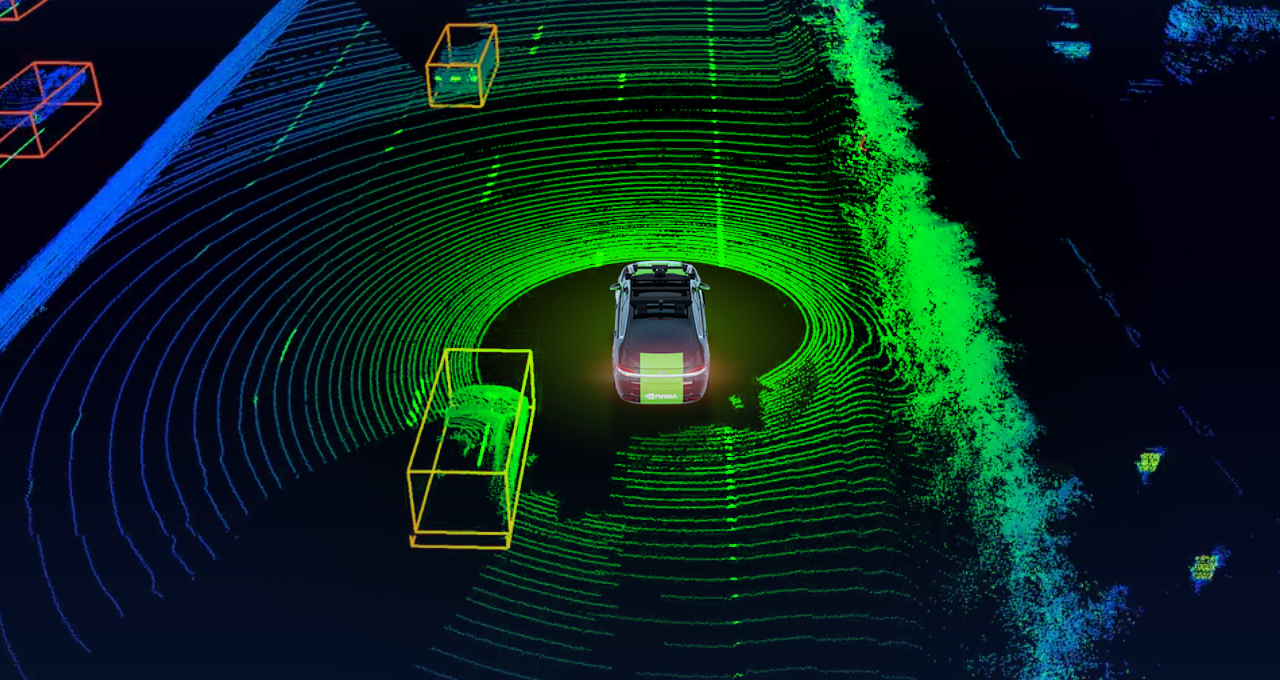
\includegraphics[width=1\linewidth]{images/visualisatie-lidar}
    \caption{Visualisatie van een LiDAR-systeem met objectherkenning in auto's~\autocite{Badoni2021}}
    \label{fig:visualisatie-lidar}
\end{figure}

\subsection{Beeldfragmenten in datavorm}\label{subsec:beeldfragmenten-als-data}
Concreet worden beelden digitaal opgeslagen in tweedimensionale tabellen van pixels, waarbij elke pixel kleurdata bevat.
De resolutie, of scherpheid, van een beeldfragment wordt vaak hierin uitgedrukt.
Zo kent een standaard Full HD (FHD)-computerscherm volgens de specificaties van~\textcite{VESA2013} een resolutie van 1920 pixels bij 1080 pixels.
Deze resolutie wordt volgens statistieken van~\textcite{ValveCorporation2024} gebruikt door meer dan de helft van haar gebruikers.
Om de kwaliteit van een beeldfragment uit te drukken wordt regelmatig gebruik gemaakt van de meeteenheid megapixels, waarbij \'e\'en megapixel \'e\'en miljoen pixels voorstelt.
Hiermee ontstaat de vaststelling dat de voorafgaande en meest gebruikte specificatie van Full HD een beeldkwaliteit van 2,1 megapixels kan weergeven aan gebruikers.

\subsubsection{Kwaliteit van hedendaags camera's}
Moderne smartphones zoals de Galaxy S24 nemen volgens~\textcite{Samsung2024} foto's aan een kwaliteit van 50 megapixels en bieden daarmee ongeveer 24 keer hogere kwaliteit dan een Full HD-computerscherm kan weergeven.
Het is hierbij belangrijk om op te merken dat het aantal megapixels niet de enige factor speelt in het bepalen van beeldkwaliteit.
Deze meeteenheid bepaalt niet alleen de totale grootte van de data dat een beeldfragment bevat, maar ook ongewenste data zoals ruis of andere artefacten.
Om het voorgenoemde fenomeen te mitigeren wordt in vele gevallen aan pixel binning gedaan, een proces waarbij pixels gegroepeerd worden tot zogenaamde superpixels~\autocite{Jin2012}.
\begin{figure}
    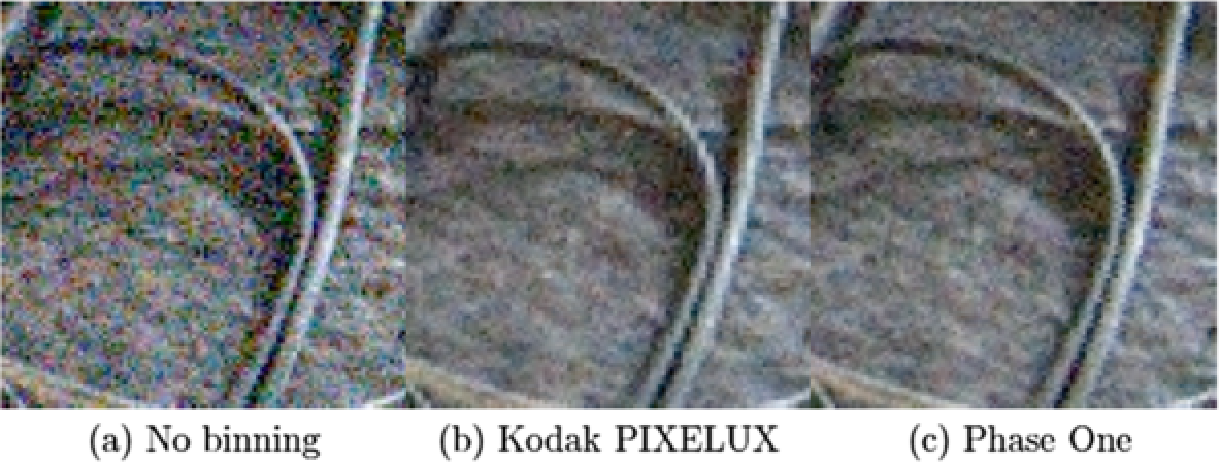
\includegraphics[width=1\linewidth]{images/pixel-binning}
    \caption{Visualisatie van pixel binning~\autocite{Jin2012}}
    \label{fig:pixel-binning}
\end{figure}


\subsection{Het verwerken van data uit multimedia}\label{subsec:het-verwerken-van-data}
Om de nauwkeurigheid en snelheid van objectherkenningsalgoritmen zo veel mogelijk te bevorderen worden eerst enkele stappen uitgevoerd ter voorbereiding.
Deze algoritmen kennen immers een langere verwerkingstijd bij grotere bestanden.
Beeldfragmenten ondergaan hiervoor verschillende processen, waaronder het voorgenoemde pixel binningsproces.

\subsubsection{Pixel binning}
Zoals eerder aangehaald kiezen moderne smartphones ervoor om pixels te groeperen in superpixels waarop vervolgens aan pixel binning gedaan wordt.
Het effect hiervan is het verzachten van observeerbare ruis, zoals zichtbaar in~\ref{fig:pixel-binning}.
Beelden die genomen zijn in donkere plekken kunnen daarmee een hogere waarneembare beeldkwaliteit krijgen.
Een bijkomend effect van dit proces is de kleinere voetafdruk van de verwerkte beelden doordat er een kleiner aantal pixels overblijven.
In het geval van smartphones wordt vaak gekozen om te binnen richting 12 megapixels, wat tussen de schermresoluties 4K Ultra HD (ongeveer 8 megapixels) en 8K Ultra HD (ongeveer 33 megapixels) ligt.
Deze resoluties worden steeds vaker gebruikt in televisies~\autocite{Statista2024}.

\subsubsection{Transformatie van beelden}
Beeldfragmenten kunnen naast pixel binning op andere manieren bewerkt worden om meer specifieke informatie te benadrukken en op te slaan.
Een voorbeeld hiervan is Fouriertransformatie, zoals beschreven in het onderzoek van~\textcite{Olaoye2024}.
Door middel van deze techniek worden dominante ruimtelijke frequenties benadrukt wat het identificeren van patronen, randen en texturen van beelden mogelijk maakt.
Beelden kunnen daarnaast ook geschaald of gedraaid worden voor geometrische correcties of ter uitlijning van afbeeldingen.
Vervolgens kunnen beelden opgedeeld worden naar gelang de kleur, textuur of randen.

\subsection{Klassieke objectherkenningsalgoritmen}
\label{subsec:klassieke-objectherkenningsalgoritmen}
Na het verwerken van beeldfragmenten komt verdere segmentatie aan bod door middel van klassieke objectherkenningsalgoritmen.
Het verschil tussen deze categorie van algoritmen en moderne objectherkenningstechnieken komt verder aan bod het hoofdstuk~\nameref{sec:datasets}.

\subsubsection{Schaalinvariante kenmerkentransformatie)}
\textcite{Tamara2022}~beschrijft Schaalinvariante kenmerkentransformatie (SIFT) als een algoritme voor het identificeren van lokale kenmerken in een afbeelding.
\begin{figure}
    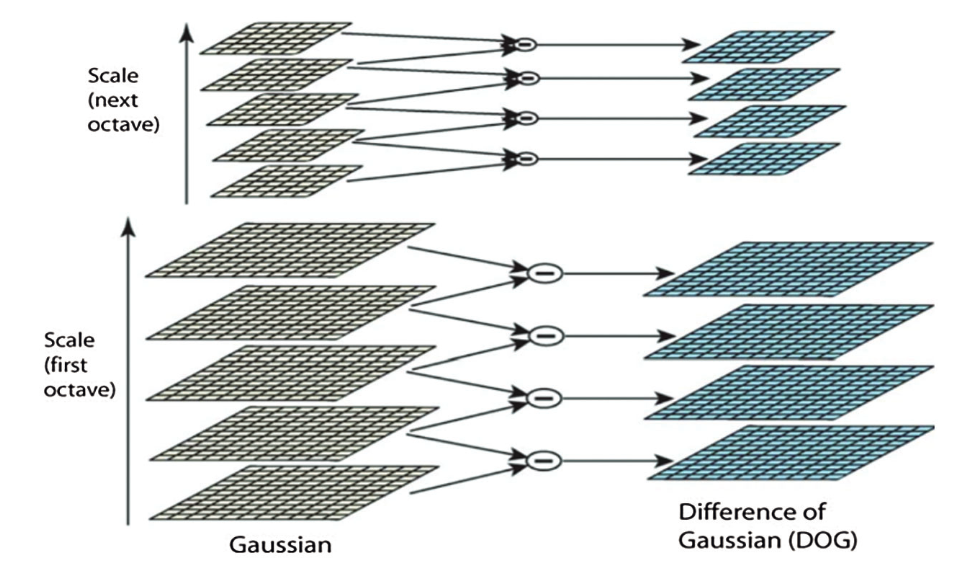
\includegraphics[width=1\linewidth]{images/DoG}
    \caption{Visualisatie van het verschil in Gaussianen~\autocite{Lowe2004}}
    \label{fig:difference-of-gaussian}
\end{figure}
Het eerste deel van dit algoritme bestaat uit het berekenen van de minima en de maxima uit het verschil in Gaussianen (DoG) met verschillende standaardafwijkingen, zoals gevisualiseerd in~\ref{fig:difference-of-gaussian}.
Daarna worden uitschieters weggefilterd door middel van een wiskundige Hessische matrix.
Een normalisatie van het aantal kenmerken kan vervolgens behaald worden door een minimum contrast van de verschillende standaardafwijkingen te hanteren.
Het toepassen van ori\"entatietoewijzing verzekert hierbij de eigenschap van rotatie-invariantie.
Uit deze stappen ontstaan enkele SIFT-beschrijvingen die vergelijking met andere afbeeldingen mogelijk maken om te bepalen of ze tot dezelfde categorie horen.
Dit gehele proces kent echter aanzienlijke verwerkingstijd waardoor het gebruik in real-time applicaties beperkt blijft.

% en het opstellen van een Histogram van Geori\"enteerde Gradi\"enten (HOG) en Lokale Binaire Patronen (LBP).
% TODO: uitdagingen en beperkingen van objectdetectie
% variaties in verlichting, complexe achtergronden, schaalvariaties, vervormingen en occlusie.

%---------- De werking van AI ----------------------------------------------------------
\section{De werking van grote taalmodellen}
\label{sec:ls-artificiele-intelligentie}
In het vorig hoofdstuk kwam computer visie aan bod als vakdomein binnen de artifici\"ele intelligentie.
Een ander, en met hedendaagse coverage in het nieuws wellicht bekendere, domein hierin is de toepassing van large language models (LLM).
Voorbeelden hiervan zijn GPT en haar toepassing ChatGPT. % TODO: hier op verder gaan & kijken naar voorstel of daar niets uit genomen kan worden.

%---------- Datasets generereren ------------------------------------------------------
\section{Het trainen van datasets voor objectherkenning}\label{sec:datasets}
Uitleg hier over: % TODO
- hoe wordt bepaald wat een geldig beeld is om mee te trainen
- hoe worden datasets getraind
- misschien statistieken van hoe nauwkeurig
- bestaande datasets gebruiken zoals Google Gemini Vertex
%  populaire datasets, zoals COCO (Common Objects in Context), Pascal VOC (Visual Object Classes), en ImageNet, worden vaak gebruikt voor het trainen en evalueren van objectherkenningsalgoritmen.